%%%%%%%%%%%%%%%%%%%%%%%%%%%%%%%%%%%%%%%%%%%%%%%%%%%%%%%%%%%
% EPFL report package, main thesis file
% Goal: provide formatting for theses and project reports
% Author: Mathias Payer <mathias.payer@epfl.ch>
%
% This work may be distributed and/or modified under the
% conditions of the LaTeX Project Public License, either version 1.3
% of this license or (at your option) any later version.
% The latest version oset ft?f this license is in
%   http://www.latex-project.org/lppl.txt
%
%%%%%%%%%%%%%%%%%%%%%%%%%%%%%%%%%%%%%%%%%%%%%%%%%%%%%%%%%%%
\documentclass[a4paper,11pt,oneside]{report}
% Options: MScThesis, BScThesis, MScProject, BScProject
\usepackage[BScThesis,lablogo]{EPFLreport}
\usepackage{xspace}
\usepackage{listings}
\usepackage{xcolor}
\usepackage{float}


\definecolor{codegreen}{rgb}{0,0.6,0}
\definecolor{codegray}{rgb}{0.5,0.5,0.5}
\definecolor{codepurple}{rgb}{0.58,0,0.82}
\definecolor{backcolour}{rgb}{0.95,0.95,0.92}

\lstdefinestyle{mystyle}{
    backgroundcolor=\color{backcolour},   
    commentstyle=\color{codegreen},
    keywordstyle=\color{magenta},
    numberstyle=\tiny\color{codegray},
    stringstyle=\color{codepurple},
    basicstyle=\ttfamily\footnotesize,
    breakatwhitespace=false,         
    breaklines=true,                 
    captionpos=b,                    
    keepspaces=true,                 
    numbers=left,                    
    numbersep=5pt,                  
    showspaces=false,                
    showstringspaces=false,
    showtabs=false,                  
    tabsize=2
}

\lstset{style=mystyle}

\title{Retrofitting defences to C++ code}
\author{Hassan Habib}
\supervisor{Nicolas Badoux}
\adviser{Prof. Dr. sc. ETH Mathias Payer}
%\coadviser{Second Adviser}
%\expert{The External Reviewer}

\newcommand{\sysname}{Retrowrite\xspace}
\newcommand{\todobox}[3]{%
    \colorbox{#1}{\textcolor{white}{\sffamily\bfseries\scriptsize #2}}%
    ~\textcolor{blue}{#3} %
    \textcolor{#1}{$\triangleleft$}%
}
\newcommand{\nb}[1]{\todobox{orange}{Nicolas:}{#1}}

\begin{document}
\maketitle
%\makededication
%\makeacks

\begin{abstract}
    The \sysname project is a static binary rewriter that allows to add
    instrumentation into programs where the source code is not available.


    \textit{C++} being a largely used programming language, we must ensure that
    progams written in this language are safe. So our task is to test \sysname on
    various \textit{Debian} packages written in \textit{C++} to see if the binary
    could be modified for instrumentation.

    From our results, we can see that \sysname worked on $38.1\%$ of packages but in
    $60.2 \%$ cases, the assembly obtained could not be compiled back to a
    functionning executable. Unforthunately, we were unable to gain more
    information about the compilation errors. Also, only a few programs encountered
    runtime errors. We have also found that file size plays a role in the
    success of \sysname. Large files seem not to be able to be
    transformed without encountering an error.
    We concluded that there is still works to do to have a fully \textit{C++} support.

\end{abstract}


\maketoc

%%%%%%%%%%%%%%%%%%%%%%
\chapter{Introduction}
%%%%%%%%%%%%%%%%%%%%%%

%The introduction is a longer writeup that gently eases the reader into your
%thesis~\cite{dinesh20oakland}. Use the first paragraph to discuss the setting.
%In the second paragraph you can introduce the main challenge that you see.
%The third paragraph lists why related work is insufficient.
%The fourth and fifth paragraphs discuss your approach and why it is needed.
%The sixth paragraph will introduce your thesis statement. Think how you can
%distill the essence of your thesis into a single sentence.
%The seventh paragraph will highlight some of your results
%The eights paragraph discusses your core contribution.
%
%This section is usually 3-5 pages.
It is unfortunately not easy to use only free software or even software whose
source code is available. This can be a security problem as it is difficult
for the community to discover new bugs. Indeed, techniques such as fuzzing or
memory sanitization can only be applied by modifying the binary file through the
compiler. Fortunately, a technique makes it possible to insert instrumentation
without having access to the source code.

Binary rewriting is a technique used in order to insert instrumentation into
binary executables where the source code is not accessible. These tools allow
the insertion of instrumentation by analyzing the executable file. They can be
categorized into two approaches: static and dynamic. The first category
generates an executable whose instrumentation could be added while the second
adds these instrumentations during the execution of the program. The first
approach has the advantage of having less impact on execution time.

Retrowrite is one most recent and successful tools. It has the advantage of
producing executables which are sound and whose overhead is almost absent.
Similarly, C/C++ are widely used languages because of their speed and the
freedom they give in memory management. Retrowrite was initially built to
support binary files written in C. Fortunately, work was then done to support
C++. Our job is therefore to test Retrowrite on several programs and try to
find cases in which it does not work as expected in order to make it available
as a robust tool.

%%%%%%%%%%%%%%%%%%%%
\chapter{Background}
%%%%%%%%%%%%%%%%%%%%
We will explain several aspects in order to allow the reader to be familiar
with any binary rewriter and more precisely \sysname. Our experience is not
exactly based on implementing or improving this tool, we still provide information
so that the reader can see the big picture regarding software that modify binary
executable.

\section{Compiler}
Computer programs can be executed in two different ways: they can be interpreted
by a software (an interpreter) or they can be compiled into machine code that can
then be executed by the hardware. 


In the first approach, the interpreter will read each line it encounters, and
then it will translate them and run them one at a time. Interpreting a program
is much slower than running the machine code generated by a compiler as we must
also run the interpreter alongside the program.

In the second approach, a compiler is needed to translate the source code into
binary code.
The compiler will analyze all the source code and generate the machine code.
Note that it will not execute the source code but only generate an executable
file.


Even if the compiled program run faster than an interpreted one, one might
prefer to write program in an interpreted language because it is platform
independant in most of the cases. And to start executing the program takes less
time if the source files were modified.



\section{Binary executable}
\texttt{C++} being a comiled langauge, we will focus on the executable file
generated by the compiler. We will now discuss the most common format of binary
executable: the \texttt{ELF} format.
\subsection{ELF format}
%source man page elf
%
The dominant executable format for binary in Unix system is the
ELF\footnote{Executable and Linkable Format} format. 


An executable file respecting the ELF format must follow a certain layout. At
first, it must have an ELF header followed by a program header table or a section
header table, or both. 
The ELF header contains the offset to the section header table and the program
header table. The program header contains information about the segments used
at runtime. The section header lets locate all the single sections of the
binary. \autoref{fig:elf} illustrates the structure of an ELF file. The
\textit{readelf}~\cite{readelfMan} command in \textit{GNU/Linux} allows us to
see the different section's information. The sections can be divided into two
categories: the predefined non-user sections and the predefined user
sections~\cite{sparc}.

\begin{figure}[H]
    \centering
    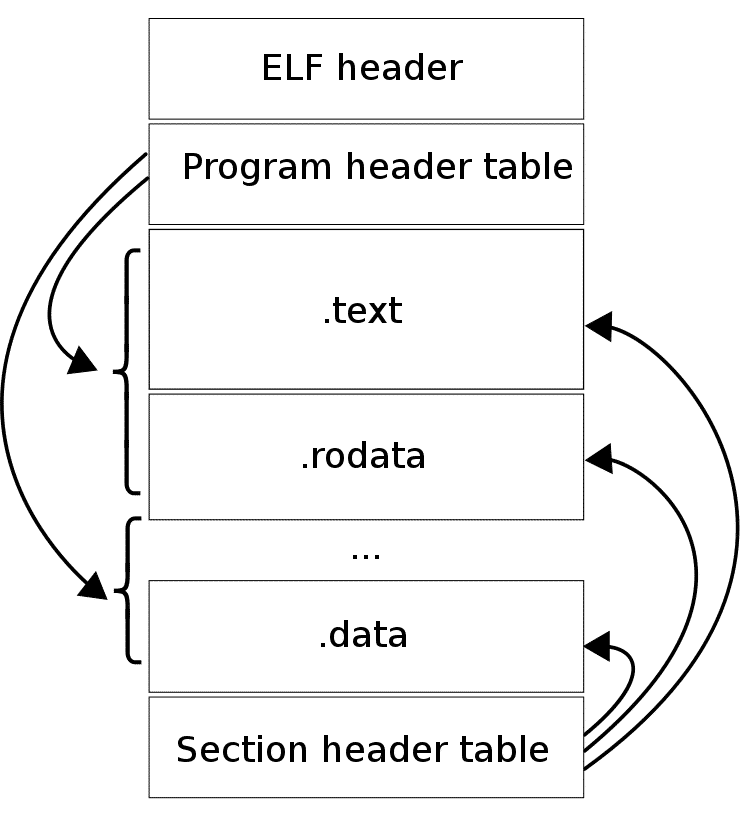
\includegraphics[width=8cm]{elf_structure.png} 
    \caption{Structure of ELF file}
    \label{fig:elf}
\end{figure}

\subsection{Predefined User Sections}
This categorie contains all sections that can be manipulated by the section
control directives.
\begin{itemize}
    \item    .bss: contains uninitialized data.
    \item    .data: contains initialised read-write data.
    \item    .debug: contains debugging information.
    \item    .rodata: contains initialised read-only data.
    \item    .text: contains the code.
\end{itemize}

\subsection{Predefined Non-User Sections}
These are all the predefined sections by the assembler.
\begin{itemize}
    \item    .dynamic: Holds all needed information for dynamic linking.
    \item    .dynstr: contains string table of .dynsym section.
    \item    .dynsym: contains symbol tables dedicated to dynamically linked
        symbols.
    \item    .got: contains the global offset table.
    \item    .interp: contains the path name of a program interpreter.
    \item    .plt: contains the procedure linkage table.
    \item    .strtab: contains string table of .symtab section.
    \item    .symtab: contains global symbol table.
\end{itemize}







\subsection{Usage}
The binary executable produced by the compiler can now be used to run the program.
Having the program in this new file does not remove the utility of the source code.
Indeed, a compiler can be executed with multiple flags in order to have a more 
specific executable. For example, a program might need to be tested before its
release.
To do so, memory errors can be discovered using a feedback-guided fuzzer
combined with sanitization.
To check the memory, a tool named \textit{Address Sanitizer} (ASan)~\cite{ASan}
can be used by compiling the source code with a certain flag that will tell the
compiler to add the instrumentation.
In the case of an end user wanting to test a closed source software, it is
nearly impossible to get the program compiled with the instrumentation needed.
Tools such as binary rewriters can be used in order to face this issue.


\section{Binary rewritting}
Binary rewritting consists of modifying an executable in the absence of source
code while maintaining functionnality. It can be used for multiple reasons as
for example for program optimization, program obfuscation or as in the case of
\sysname for security policy enforcement via instrumentation. 


Binary rewriters can be divided into two main approaches: dynamic
instrumentation and static instrumentation.

\subsection{Dynamic instrumentation}
%%executer virtuellement le programe
In this scheme, the rewritting is done while the program is executed. Usually
the binary is executed side by side with the rewriter engine. In order to
analyze and interact with the program during the execution. The rewriter might
use the OS's primitves as the PTRACE API in Linux for example.  An advantage of
dynamic instrumentation is that analyzing the whole binary might be avoided.
This is practical for large binaries. However, the disadvantage of using this
technique is the high performance cost. Translating the program at runtime does
not come with no cost and the overhead is way higher than running a modified
binary executable~\cite{dinesh20oakland}.


\subsection{Static instrumentation}
Contrary to dynamic instrumentation, static rewriters operates on binaries
at static time. It outputs a new binary executable that corresponds to the
initial executable but rewritten. This generated executable have the advantage
of being almost as fast as the original executable that would have been
compiled for instrumentation as the overhead introduced are usually low.


\subsection{Steps in binary rewritting}
Both dynamic and static instrumentation follow four main steps:
\begin{enumerate}
    \item Parsing:
        This step consist of obtaining the instruction stream from the binary
        and pass it to a disassembler.
    \item Analysis:
        This part consists of gaining as much information as possible. The
        objectif is to recover the structure of the source code.
    \item Transformation:
        Here, we must find all the locations where instrumentation must be
        added or removed. 
    \item Code generation:
        We have to make sure that adding the instrumentation does not modify the
        behaviour of the executable. The modified executable must be sound. And
        then the original executable must be patched or new executable must be
        generated.
        There are multiple techniques for this part. 
\end{enumerate}



\subsection{Transformation and Code genreation techniques}
There are multiples techniques for the transformation and code generation
parts. The simplest technique is called \textit{Trampoline}. All new code are
added in new sections in the binary. Branches are then added to redirect to the
right location after an instrumentation point. This technique introduce too much overhead as we
need to jump from and to the trampoline at each instrumentation. 


Another technique is named \textit{Direct}. This is one of the oldest
technique. Here the code is simply overwritten. We have to make sure to reajust
every branch and references.  But this technique does not scale well as adding
and removing instructions implies an update of all branch targets.


The technique used by \sysname is called \textit{Symbolization}. It
consists of transforming the binary into an assembly text file. It transforms
all references constants into assembly labels. Then, many tools can insert
instrumentation into the reassembled file. Unlike the trampoline technique,
this method is defined as being \textit{zero-overhead} as the only overhead
added is the time to execute the instrumentation.
%add example of symbolization

\section{Retrowrite}
%link to paper
Retrowrite~\cite{dinesh20oakland} is a binary rewriter developped by HexHive.
It uses the symbolization technique by generating re-assembleable assembly.
Retrowrite has as objectif to be sound by the way they determine reference
constants and symolize them. It uses
\textit{Capstone} as a disassembler and \textit{pyelftools} as a binary parser.

\section{Other security techniques}
\textit{C/C++} are two of the most used programming languages. They are
mainly used for their runtime performance and low level memory access
capabilities, but this comes with a cost. In these languages, memory and type
safety are managed by the programmers. Tools can be used to enforce the safety
of software. For example, one might want to use \textit{HexType} to enforce
type safety.

\subsection{HexType}
\textit{HexType} is a tool written by the \textit{HexHive} lab in order to
detect type confusion in software written in \textit{C++}. Typecast are when a
pointer of a certain type is converted into antoher. Typecast are
normally checked statically. The vulnerability lies in the fact that
down-casting is allowed. Down-casting means transforming a pointer representing
a class into one of its descendants as seen in the code example. This can lead
to type confusion as no one prevents the program to cast an object of
incompatible base type. \textit{HexType} remedy to this issue by transforming
static checks to runtime checks.

\lstinputlisting[language=C++]{type_confusion.cpp}



%%%%%%%%%%%%%%%%
\chapter{Goal}
%%%%%%%%%%%%%%%%
As stated in their paper~\cite{dinesh20oakland}, \textit{Retrowrite} was
firstly designed to support Linux x86-64 PIC binaries that were written in the
\textit{C Programming Language}. The main obstacle for adding support for
\textit{C++} is that the symbolization of C++ exception
handlers is not yet supported. Multiple works were done in order to add support
for C++ as it can be seen in the \textit{Retrowrite} repository~\cite{gitCommit}.


\section{Challenges}
When Retrowrite was presented to the public, C++ was not yet fully supported.
But C++ being a more versatile language than C, it seemed obvious that the
support of the latter was essential to make Retrowrite a complete tool. Our
first intention was to integrate hextype into retrowrite. But then it turned
out that the task was more difficult than expected. Since not having the source
code, it was complicated to obtain the information on the classes. It would be
possible to do something if debugging information was available, but this is
not the case for many executables. Similarly, pyelftools cannot analyze
executables with a version of gdwarf < 4.0, whereas the standard is version 5
today.

Then, \textit{Hexhive} released a version of retrowrite on their repository
where C++ support was added. So we decided to focus on testing this new
feature.
We focused on testing \sysname on as many packages as possible but didn't
really pay attention to whether the modified file behaved like the original
file.

\section{Task}
The task was to test many packages from the
\textit{Debian}~\cite{debian} distribution. Debian being a widely used
distribution, we thought it would be a good idea to use it as a source. 
We tested Retrowrite on a bunch of programs that can be found on Debian.
The test were not extensive as we were only testing if the command
\textit{--help} worked. The purpose of the testing was to see if the compiler
was able to compile the assembly file generated by \sysname.


%%%%%%%%%%%%%%%%%%%%%%%%
\chapter{Implementation}
%%%%%%%%%%%%%%%%%%%%%%%%

The main script is \textit{clone.sh}. It will start several containers which will
each take care of one package. This script also takes care of running the
command that will prepare the results.

\section{Docker}
The first decision was to test \textit{Retrowrite} in
\textit{docker}~\cite{merkel2014docker} containers. This allows us to emulate
\textit{Debian} on any machine. Each container will execute
\textit{entrypoint.sh} on a specific package. The binaries available from the
command \textit{apt install}~\cite{apt} are stripped, so we had to download the
source code and compile the program ourselves. Then we ran the program with the
argument "\textit{--help}" and compared the exit code with the recompiled
program from the assembly file re-assambled by retrowrite. The programs are
then sorted according to their output code.


\section{Linking}
One problem encountered was recompiling the
assembly files by linking them to the correct shared-libraries. To do so, a 
script was written called  \textit{flib.sh} which takes as argument the original binary
file. It will then return, using the command "ldd"\cite{ldd} the list of
libraries to link. 

\section{List of packages}

Having obtained a list of packages from the Debian distribution
\cite{sourcePackage}, we needed a way of filtering to only obtain
a list of packages written in \textit{C++}. To do this, we use the script
\textit{filter\_c++\_packages.sh}. It will simply look in the information given
in \textit{apt show}~\cite{apt} if the package was written in \textit{C++} or
not. 

\section{Filtering the result}
When the docker containers have finished executing their commands, the
\textit{result\_count.sh} script will be executed. This script takes care of searching
and sorting the results by arranging them and putting them in a new folder.
%explain the categories when it is more clear

\section{Use of exceptions}
We also needed a way to find which binaries were using exception. Using
pyelftools, we noticed that all binary files using exceptions also had a call
instruction to \verb|__cxa_begin_catch@plt| function or
\verb|__cxa_allocate_exception@plt|, both in the plt section. So we just looked
in the \textit{.rela.plt} section and search for the
\verb|__cxa_allocate_exception| symbol. The script is named
\textit{elfexceptions.py}


All the scripts used can be found in the GitHub
\href{https://github.com/ha2san/debian_docker/tree/main/scripts}{repository}~\cite{repo}.

%%%%%%%%%%%%%%%%%%%
\chapter{Evaluation}
%%%%%%%%%%%%%%%%%%%

In \autoref{table:popular}, you can see the result of our scripts on the most
popular pacakges in \textit{Debian}. The \autoref{table:remaining}
corresponds to the remaining packages found in other list. The
\textit{discard} line corresponds to the packages where the program was not
testable. Running them with \textit{--help} leads to a crash or an error. 
The category "\textit{unsuccessful compilation}" means that we were not able to
compile the re-assembled assembly back to an executable for various reason as
missing shared-libraries or the assembly file contains some error. It was not
possible to categorize these errors as \textit{clang} always outputs the same
error in each situation: "\texttt{<unknown>:0: error: Undefined temporary symbol .L26312 }".
The "\texttt{runtime error}" category corresponds to when we succeed to run
the modified executable but a segmentation fault was encountered.


\begin{table}[H]
    \centering
    \begin{tabular}{lll}
        \hline
        category                & \#packages & percentage\\
        \hline
        discard                  & 302 & - \\
        no errors                & 243 & 40.0\% \\
        unsuccessful compilation & 349 & 57.4\% \\
        runtime error            & 16  & 2.6\% \\
        \hline
        total                    & 910  \\ 
        \hline
    \end{tabular}
    \caption{Popular packages}
    \label{table:popular}
\end{table}


\begin{table}[H]
    \centering
    \begin{tabular}{lll}
        \hline
        category                & \#packages & percentage \\
        \hline
        discard                  & 109 & -  \\
        no crash                 & 172 & 35.8\% \\
        unsuccessful compilation & 306 & 63.7\% \\
        runtime error            & 2   & 0.41\% \\
        \hline
        total                    & 589  \\
        \hline
    \end{tabular}
    \caption{Remaining packages}
    \label{table:remaining}
\end{table}

As you can see in thes figures, the most dominant category is the
"\textit{unsuccessful compilation}" one. Only a few programs crashed during the
runtime. This is a nice result as \sysname claims that the code produce is
sound.

By reading the \sysname paper~\cite{dinesh20oakland}, we understand that
the biggest issue with adding \textit{C++} support was to handle symbolization
of exception handlers. It seems that is not yet fully supported as testing a
simple program using exception leads to a runtim error:

\lstinputlisting[language=C++]{exception.cpp}

Retrowrite succeeded to rewrite the executable but running it leads to a segmentation fault.
We wanted to see for all the packages, which one fails and was using
exceptions. The result can be seen in \autoref{table:exception}.

As you can see, most of the segmentation fault were encountered with programs
using exception. The difference is not that big, but we see that the compilation
was more successful when the program was using exceptions. We understand from
the test done that the program crahses only if he gets in a catch clause.

\begin{table}[H]
    \centering
    \begin{tabular}{lll} 
        \hline
        category                & \#packages & percentage \\ 
        \hline
        crash during compilation & 199 & 64.6\%      \\
        no crash                 & 92  & 29.9\%       \\
        crash during runtime     & 17  & 5.5 \%       \\
        \hline
    \end{tabular}
    \caption{Packages using exception}
    \label{table:exception}
\end{table}


\begin{table}[H]
    \centering
    \begin{tabular}{lll} 
        \hline
        category                & \#packages & percentage \\ 
        \hline
        crash during compilation & 427  & 57.2\%      \\
        no crash                 & 318  & 42.6\%      \\
        crash during runtime     & 1    & 0.1\%      \\
        \hline
    \end{tabular}
    \caption{Packages not using exceptions}
\end{table}

Another observation that can be made is that the size of the executable
matters. As you can see in \autoref{fig:sizes}, the number of executables that
could be compiled and run drops drastically to 0 as the file size increases. In
the other direction, the number of errors at the compilation level rises in
parallel to the size of the file. Similarly, the number of runtime errors also
increases with file size, but we believe this is more related to exception
usage.

Take into consideration that the file sizes shown here correspond to stripped
executables. But we used \sysname on their non-striped versions.
Unfortunately, we no longer had the unstriped versions and recompiling each
package would have taken us too long. These figures given are therefore only
representative.

\begin{figure}[H]
    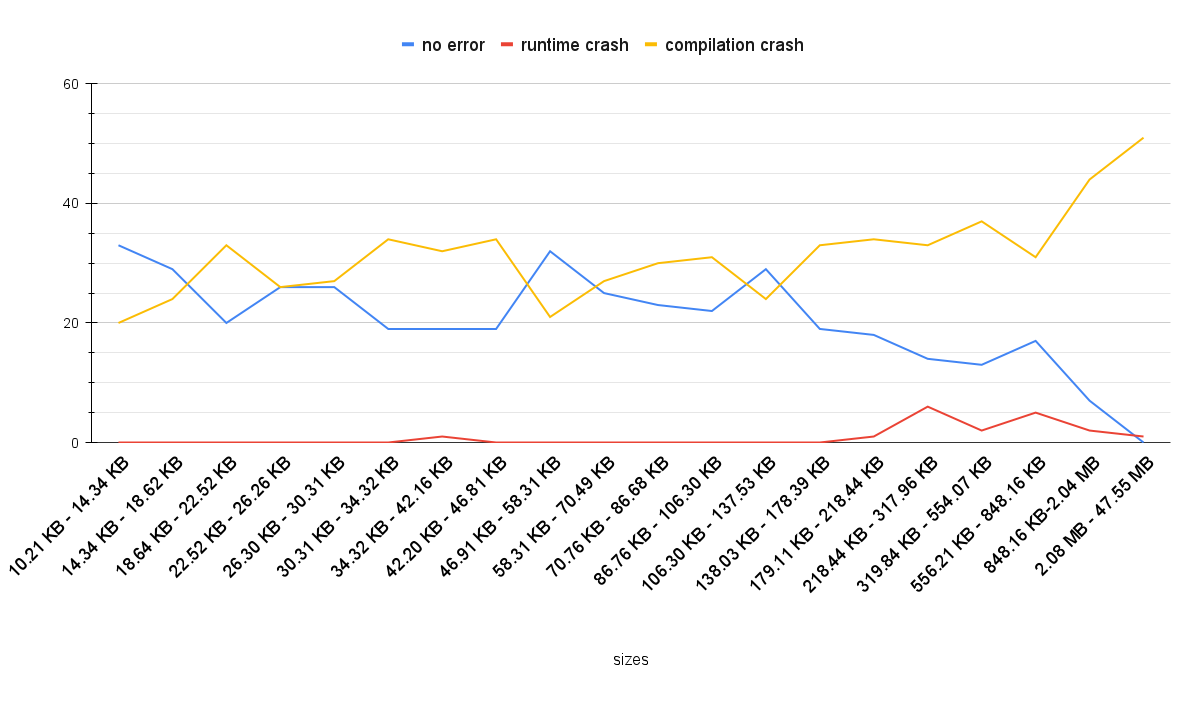
\includegraphics[width=\linewidth]{chart.png} 
    \caption{classification of packages according to their size}
    \label{fig:sizes}
\end{figure}

\begin{table}[H]
    \begin{tabular}{llll}
        \hline
        sizes               & \multicolumn{1}{l}{no error} & \multicolumn{1}{l}{runtime crash} & \multicolumn{1}{l}{compilation crash} \\
        \hline
        10.21 KB-14.34 KB   & 33                           & 0                                 & 20                                    \\
        14.34 KB-18.62 KB   & 29                           & 0                                 & 24                                    \\
        18.64 KB-22.52 KB   & 20                           & 0                                 & 33                                    \\
        22.52 KB-26.26 KB   & 26                           & 0                                 & 26                                    \\
        26.30 KB-30.31 KB   & 26                           & 0                                 & 27                                    \\
        30.31 KB-34.32 KB   & 19                           & 0                                 & 34                                    \\
        34.32 KB-42.16 KB   & 19                           & 1                                 & 32                                    \\
        42.20 KB-46.81 KB   & 19                           & 0                                 & 34                                    \\
        46.91 KB-58.31 KB   & 32                           & 0                                 & 21                                    \\
        58.31 KB-70.49 KB   & 25                           & 0                                 & 27                                    \\
        70.76 KB-86.68 KB   & 23                           & 0                                 & 30                                    \\
        86.76 KB-106.30 KB  & 22                           & 0                                 & 31                                    \\
        106.30 KB-137.53 KB & 29                           & 0                                 & 24                                    \\
        138.03 KB-178.39 KB & 19                           & 0                                 & 33                                    \\
        179.11 KB-218.44 KB & 18                           & 1                                 & 34                                    \\
        218.44 KB-317.96 KB & 14                           & 6                                 & 33                                    \\
        319.84 KB-554.07 KB & 13                           & 2                                 & 37                                    \\
        556.21 KB-848.16 KB & 17                           & 5                                 & 31                                    \\
        848.16 KB-2.04 MB   & 7                            & 2                                 & 44                                    \\
        2.08 MB-47.55 MB    & 0                            & 1                                 & 51    \\                               
        \hline
    \end{tabular}
\end{table}

During our tests, we were able to discover some problems and reported them to
the developers. The first being that some assembly files can only be
transformed into executable format using clang and not gcc. Another issue was
that the compiler seemed to not recognize certain sections in the assembly
file. A solution was then offered in the comments when the issue was written
where a user simply proposed to remove all references to these sections.


%%%%%%%%%%%%%%%%%%%%
\chapter{Conclusion}
%%%%%%%%%%%%%%%%%%%%

In general, \sysname worked on a lot of packages, and we encountered few runtime
errors. The main problem was that it was not possible to compile the
re-assembled assembly back on most of the packages. The results also showed
that \sysname can not hanlde exceptions yet. Similarly, \sysname seems to
encounter errors with large file sizes. We also had to find the shared-libraries
ourselves. It would be an enhancement if retrowrite could do it for x86 CPU as
it seems that this option is only available for \textit{ARM}
cpu~\cite{retroArm}.

\cleardoublepage
\phantomsection
\addcontentsline{toc}{chapter}{Bibliography}
\printbibliography

% Appendices are optional
% \appendix
% %%%%%%%%%%%%%%%%%%%%%%%%%%%%%%%%%%%%%%
% \chapter{How to make a transmogrifier}
% %%%%%%%%%%%%%%%%%%%%%%%%%%%%%%%%%%%%%%
%
% In case you ever need an (optional) appendix.
%
% You need the following items:
% \begin{itemize}
% \item A box
% \item Crayons
% \item A self-aware 5-year old
% \end{itemize}

\end{document}
